Ao longo dos próximos capítulos quando for necessário elaborar algum exemplo de aplicação utilizando a biblioteca TivaWare, o hardware ao qual se destinará o exemplo será o microcontrolador  Tiva \texttrademark ~~ TM4C1294NCPDT, um kit de desenvolvimento da empresa Texas Instruments que possui um microcontrolador baseado no processador ARM Cortex-M4. Porém quando o dado exemplo for elaborado utilizando a biblioteca CMSIS, o hardware correspondente será o microcontrolador MSP432P401R\texttrademark, outro kit de desenvolvimento da Texas Instruments, que também possui um processador ARM Cortex-M4.  

A Tabela \ref{tab:CaracteristicasMicroTiva} traz as principais características do microcontrolador Tiva \texttrademark. 

%% TABELA DE CARACTERISTICAS BASICAS Tiva %%%%%%%%%%

\begin{longtable}{|l|l|}
	\hline
	\cellcolor[HTML]{343434} \color[HTML]{FFFFFF} Características & \cellcolor[HTML]{343434} \color[HTML]{FFFFFF} Descrição \\
	\hline
	Núcleo & ARM Cortex-M4F\\
	\hline
	Performance & Operação até 120-MHz; 150 DMIPS \\
	& (Dhrystone MIPS) de performance \\
	\hline
	Memória Flash & 1024 KB  \\
	\hline
	SRAM & 256 KB single-cycle System SRAM \\
	\hline
	EEPROM & 6KB  \\
	\hline
	ROM & ROM interna carregada com biblioteca  \\
	 & TivaWare™  C Series \\
	\hline
	Interface de Periféricos Externos (EPI)  & Interface dedicada de 8-/16-/32-   \\ 
	 &  bits dedicados a periféricos e memoria\\
	\hline
	 Verificação de Redundância & Função Hash de 16-/32- bits,  que suporta  \\
	  Cíclica (CRC)   & quatro formas de CRC \\
	\hline
	Universal Asynchronous  & 8 módulos UARTs \\
	Receivers/Transmitter (UART) & \\
	\hline
	Quad Synchronous Serial & Quatro módulos de SSI com Bi- , Quad-\\
	Interface (QSSI) &  e suporte avançado de SSI\\
	\hline
	Inter-Integrated Circuit ($I^{2}C$) & 10 módulos $I^{2}C$ com 4 velocidades \\
	 & de transmissão\\
	\hline
	Controller Area Network (CAN) & 2 controladores CAN 2.0 A/B \\
	\hline
	Ethernet MAC & 10/100 Ethernet MAC \\
	\hline
	Ethernet PHY & PHY com IEEE 1588 PTP \\
	\hline
	Universal Serial Bus (USB) & USB 2.0 OTG/Host/Device  \\ 
	& com ULPI interface e suporte a Link   \\
	& Power Management (LPM) \\
	\hline
	Micro Acesso Direto à Memória ($\mu DMA$) & Controlador ARM PrimeCell  \\
	& 32-channel configurável  $\mu DMA$ \\
	\hline
	General-Purpose Timer (GPTM) & 8 blocos 16/32-bit GPTM \\
	\hline
	Watchdog Timer (WDT) & 2 Watchdog Timers \\
	\hline
	Hibernation Module (HIB) & Low-power battery-backed \\
	 & Hibernation module \\
	\hline
	General-Purpose Input/Output (GPIO) & 15 physical GPIO blocks \\
	\hline
	Pulse Width Modulator (PWM) & 1 modulo PWM , com 4 geradores PWM  \\
	 & e um  registador de controle,\\
	 &  com um total de 8  saídas PWM.\\
	\hline
	Quadrature Encoder Interface (QEI) & Um modulo QEI \\
	\hline
	Analog-to-Digital Converter (ADC) & 2 modulos ADC de 12-bit\\
	 & taxa de 2 milhões de amostras/segundo\\
	\hline
	Controlador Comparador Analógico & Três comparadores analógicos \\
	& independentes \\
	\hline
	Comparador Digital & 16 comparadores digitais \\
	\hline
	JTAG e Serial Wire Debug (SWD) & 1 modulo JTAG  com ARM SWD\\
	& integrado \\
	\hline
	Encapsulamento & 128-pin TQFP \\
	\hline
	Temperatura de Operação & $-40 \degree C$ até $105 \degree C$ \\
	\hline
	\caption{Características Básicas - TM4C1294NCPDT \cite{DATASHEET_Tiva}}
	\label{tab:CaracteristicasMicroTiva}
\end{longtable}

Já a Tabela \ref{tab:CaracteristicasMicroMSP} traz as características do microcontrolador MSP432P401R\texttrademark.

%%%%%%%%%%%%%%%%%%%%%%%%%%%%%%%%%%%%%%%%%%%%%%%%%%%%%%%

%% TABELA DE CARACTERISTICAS BASICAS MSP432 %%%%%%%%%%


\begin{longtable}{|l|l|}
	\hline
	\cellcolor[HTML]{343434} \color[HTML]{FFFFFF} Características & \cellcolor[HTML]{343434} \color[HTML]{FFFFFF} Descrição \\
	\hline
	Núcleo 			& ARM Cortex-M4F\\
	\hline
	Performance 	& Operação até 48-MHz; 58.56 DMIPS  \\
	\hline
	Memória Flash 	& 256 KB  \\
	\hline
	SRAM 			& 64KB \\
	\hline
	ROM 			&  32KB,  contendo\\
					& biblioteca de \emph{driver} de periféricos\\
	Universal Asynchronous  & 4 módulos UARTs \\
	Receivers/Transmitter (UART) & \\
	\hline
	IrDA 			& 4 módulos de codificação e\\
					& decodificação \\
	\hline
	SPI 			& 4 módulos, com clock máximo\\
					& de 16 MHz\\
	\hline
	$I^2C$ 			& 4 módulos, com múltiplo endereçamento \\
					& de escravos.\\
	\hline
	Alimentação Variável &  No minimo 1.62 V até 3.7 V\\ 
	\hline
	LPM3                 & Consumo típico de 660 nA \\
	\hline
	LPM3.5               & Consumo típico de 630 nA \\
	\hline
	LPM4                 & Consumo típico de 500 nA \\
	\hline
	LPM4.5               & Consumo típico de 25 nA \\
	\hline
	Watchdog Timer (WDT) & 1 módulo Watchdog Timer \\
	\hline
	Suporte a Cristal de & Frequência padrão de 32.768 kHz \\
	Baixa Frequência     &                         \\
	\hline
	Suporte a Cristal de & Frequência padrão de 48 MHz \\
	Alta Frequência      &                         \\
	\hline
	RTC                  & Com funções de alarme  \\
	                     & calendário             \\
	\hline
	General-Purpose Input/Output (GPIO) & 48 Pinos de entrada/saída\\
	                                    & com capacidade de despertar \\
	                                    & 24 pinos com capacidade de mapeamento\\
		
	\hline
	Analog-to-Digital Converter (ADC) &  ADC de 14-bit\\
									  & taxa de 2 milhões de amostras/segundo\\
	\hline
	Controlador Comparador Analógico & 2 comparadores analógicos \\
								     & independentes \\
	\hline
	Temperatura de Operação & $-40 \degree C$ até $85 \degree C$ \\
	\hline
	\caption{Características Básicas - MSP432P401R\texttrademark \cite{DATASHEET_MicroMSP}}
	\label{tab:CaracteristicasMicroMSP}
\end{longtable}

%%%%%%%%%%%%%%%%%%%%%%%%%%%%%%%%%%%%%%%%%%%%%%%%%%%%%%%

O TM4C1294NCPDT possui dois barramentos. Um desses é responsável pela conexão padrão entre o núcleo de processamento e os periféricos, o \emph{Advanced Peripheral Bus} (APB). Já o outro, o \emph{Advanced High-Performance Bus} (AHB), é um barramento especial que pode ser requisitado da maioria dos periféricos. Sendo que este possui uma resposta muito mais rápida por ser exclusivo. O esquema dos barramentos é mostrado no diagrama de blocos da figura \ref{fig:DiagramaBlocosTiva}.


\begin{figure}[H]
\centering
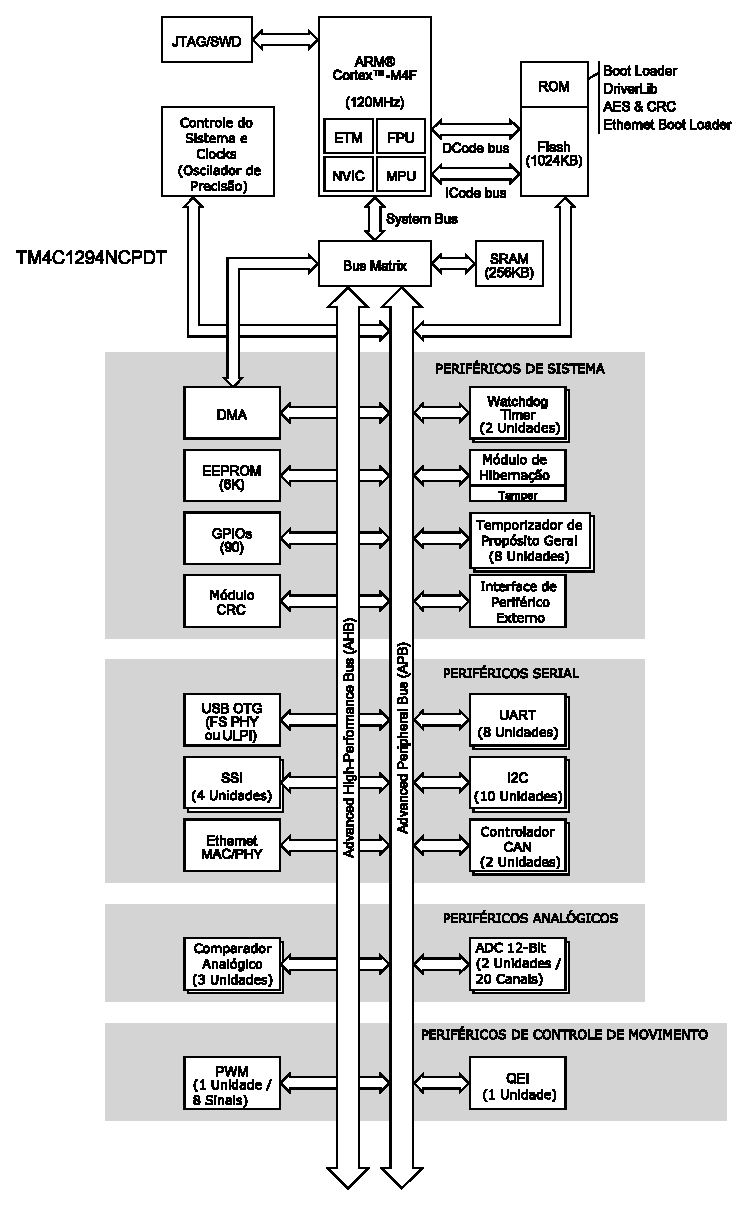
\includegraphics[width=0.6\textwidth] {DiagramaBlocosTiva.eps}
    \caption{Diagrama de Blocos - TM4C1294NCPDT \cite{DATASHEET_Tiva}}
    \label{fig:DiagramaBlocosTiva}
\end{figure}

A Figura \ref{fig:DiagramaBlocosMSP432} apresenta o diagrama de blocos do funcionamento do microcontrolador MSP432P401R\texttrademark, representando todos os periféricos e a CPU do microcontrolador de forma resumida.  Este microcontrolador não possui um \emph{Advanced High-Performance Bus}, mas sim dois barramentos simples, sendo um de dados (\emph{Data})  e outro de endereçamento (\emph{Address}). 

\begin{figure}[H]
	\centering
	\includegraphics[width=0.9\textwidth] {figuras/MSP432P401R-Diagrama.pdf}
	\caption{Diagrama de Blocos - MSP432P401R\texttrademark \cite{DATASHEET_MicroMSP}} 
	\label{fig:DiagramaBlocosMSP432}
\end{figure}